\documentclass[10pt,aspectratio=169]{beamer}

% All the boilerplate is in deslides.sty
\usepackage{deslides}

\author{Ji\v{r}\'i Lebl}

\institute[OSU]{%
Oklahoma State University%
%Departemento pri Matematiko de Oklahoma {\^S}tata Universitato%
}

\title{26. Transforms of derivatives and ODEs, part 2\\(Notes on Diffy Qs, 6.2)}

\date{}

\begin{document}

\begin{frame}
\titlepage

%\bigskip

\begin{center}
The textbook: \url{https://www.jirka.org/diffyqs/}
\end{center}
\end{frame}

\begin{frame}
Consider a constant coefficient linear differential equation
$L x = f(t)$.

\medskip
\pause

Consider $f(t)$ the input and $x(t)$ the output.

\medskip
\pause

We want a way to analyze outputs for all sorts of inputs (but same $L$).
E.g., we want to understand how a specific circuit responds to different
inputs.

\medskip
\pause

Consider the initial conditions are zero.

\medskip
\pause

Taking the Laplace transform the equation becomes
\[
A(s) X(s) = F(s) .
\]
\pause
The ratio $\frac{X(s)}{F(s)} = \frac{1}{A(s)}$ is called the
\emph{transfer function} and we denote it by $H(s)$.
\pause
So
\[
X(s) = H(s) F(s) .
\]
The output $X(s)$ is just a multiplication away
from the input $F(s)$.

\medskip
\pause

Moreover, as 
$H(s) = \frac{X(s)}{F(s)}$, we need to simply know the output $X(s)$ for one input
$F(s)$ to find the output for all inputs.
\pause
We don't even need to know $L$ itself, just its output.
\end{frame}

\begin{frame}
\textbf{Example:}
Consider $x'' + \omega_0^2 x = f(t)$ (zero initial conditions).

\medskip
\pause

Laplace transform the equation:
\[
s^2 X(s) + \omega_0^2 X(s) = F(s) .
\]
\pause
The transfer function is
\[
H(s) = \frac{X(s)}{F(s)} = \frac{1}{s^2 + \omega_0^2} .
\]
\pause
So if the input is the constant $f(t)=1$, then $F(s)=\nicefrac{1}{s}$.

\medskip
\pause

Then the output is
\[
X(s) = H(s) F(s) = \frac{1}{s^2+\omega_0^2} \, \frac{1}{s} .
\]
\pause
The inverse Laplace transform gives
\[
x(t) = \frac{1-\cos(\omega_0 t)}{\omega_0^2} .
\]
\pause
For any other input $f(t)$, the output (in $s$-space) is again simply
\[
X(s) = H(s) F(s) = \frac{1}{s^2+\omega_0^2} \, F(s) .
\]
\end{frame}

\begin{frame}
Laplace also deals with integrals easily.

\medskip
\pause

Applying the definition and a little bit of calculus gives
the property
\[
\mathcal{L} \left\{
\int_0^t f(\tau) \, d\tau
\right\} = \frac{1}{s} \, F(s)
\pause
\qquad
\text{or perhaps}
\qquad
\int_0^t f(\tau) \, d\tau
=
{\mathcal{L}}^{-1} \left\{
\frac{1}{s} \, F(s) \right\} .
\]
\pause
\textbf{Example:}
\[
{\mathcal{L}}^{-1} \left\{
\frac{1}{s(s^2+1)} \right\} 
\pause
=
{\mathcal{L}}^{-1} \left\{
\frac{1}{s} \, \frac{1}{s^2+1} \right\} 
\pause
=
\int_0^t 
{\mathcal{L}}^{-1} \left\{
\frac{1}{s^2+1} \right\} \, d\tau
\pause
=
\int_0^t 
\sin \tau \, d\tau
\pause
=
1 - \cos t .
\]
\end{frame}

\begin{frame}
An equation containing integrals is called an \emph{integral equation}.

\medskip
\pause

\textbf{Example:}
Consider we wish to solve for $x(t)$ in
\[
x(t) - t = \int_0^t x(\tau) \, d\tau .
\]
\pause
Apply the Laplace transform.  Remember
$\mathcal{L} \left\{
\int_0^t f(\tau) \, d\tau
\right\} = \frac{1}{s} \, F(s)$.
\[
X(s) - \frac{1}{s^2} = \frac{1}{s} X(s) .
\]
\pause
So
\[
X(s) = \frac{1}{s(s-1)} \pause = \frac{1}{s-1} - \frac{1}{s} .
\]
\pause
The inverse Laplace transform gives
\[
x(t) = e^t - 1 .
\]
\end{frame}

\begin{frame}
How about periodic functions?  That is, an $f(t)$ where $f(t) = f(t+P)$ for some $P$ (the period).

\pause
\medskip

$\displaystyle
F(s)
= \int_0^\infty e^{-st} f(t) \, dt
\pause
= \int_0^P e^{-st} f(t) \, dt
+ \int_P^\infty e^{-st} f(t) \, dt
$

\pause
\medskip

$\displaystyle
\phantom{F(s)}{} = \int_0^P e^{-st} f(t) \, dt
+ \int_0^\infty e^{-s(t+P)} f(t+P) \, dt
\pause
= \int_0^P e^{-st} f(t) \, dt
+ e^{-Ps} \int_0^\infty e^{-st} f(t) \, dt
$

\medskip
\pause

$\displaystyle
\phantom{F(s)}{} = \int_0^P e^{-st} f(t) \, dt
+ e^{-Ps} F(s)$.

\pause
Solve for $\displaystyle F(s)
\pause
=
\frac{1}{1-e^{-Ps}}
\int_0^P e^{-st} f(t) \, dt .
$

\medskip
\pause

\textbf{Example:}
Suppose $f(t)$ is a \emph{sawtooth}, that is,

$f(t) = t$ for $0 \leq t < 1$
and $f(t)=f(t+1)$.

\pause
So
$f(t) = t-1$ for $1 \leq t < 2$, 

$f(t) = t-2$ for $2 \leq t < 3$, etc.

\vspace*{-1.5in}
\hfill
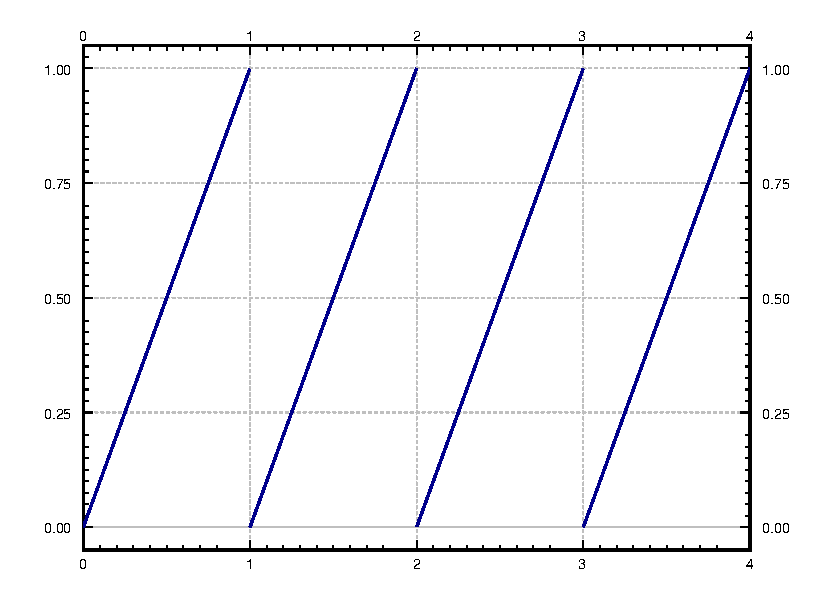
\includegraphics[width=2.5in]{figures/sawtoothfig}

\vspace*{-0.25in}

\pause
Then $P=1$ and
\[
F(s) =
\frac{1}{1-e^{-s}}
\int_0^1 e^{-st} t \, dt 
\pause
=
\frac{1}{1-e^{-s}}
\left(
\frac{-e^{-s}}{s}-\frac{e^{-s}}{s^2} + \frac{1}{s^2}
\right)
\pause
=
\frac{-e^{-s}}{(1-e^{-s})s} + \frac{1}{s^2} .
\]
\end{frame}


\end{document}
